
\chapter{A tour of IPython}

One of Python's most useful features is its interactive interpreter.
This system allows very fast testing of ideas without the overhead
of creating test files as is typical in most programming languages.
In scientific computing, one of the reasons behind the popularity
of systems like Matlab~\texttrademark, IDL~\texttrademark or Mathematica~\texttrademark,
is precisely their interactive nature. Scientific computing is an
inherently exploratory problem domain, where one is rarely faced with
writing a program against a set of well-defined explicit constraints.
Being able to load data, process it with different algorithms or test
parameters, visualize it, save results, and do all of this in a fluid
and efficient way, can make a big productivity difference in day to
day scientific work. Even for the development of large codes, a good
interactive interpreter can be a major asset, though this is a less
commonly held view; later in this document we will discuss this aspect
of the problem.

However, the interpreter supplied with the standard Python distribution
is somewhat limited for extended interactive use. The IPython project
\cite{IPython} was born out of a desire to have a better Python interactive
environment, which could combine the advantages of the Python language
with some of the best ideas found in systems like IDL or Mathematica,
along with many more enhancements. IPython is a free software project
(released under the BSD license) which tries to:

\begin{enumerate}
\item Provide an interactive shell superior to Python's default. IPython
has many features for object introspection, system shell access, and
its own special command system for adding functionality when working
interactively. It tries to be a very efficient environment both for
Python code development and for exploration of problems using Python
objects (in situations like data analysis).
\item Serve as an embeddable, ready to use interpreter for your own programs.
IPython can be started with a single call from inside another program,
providing access to the current namespace. This can be very useful
both for debugging purposes and for situations where a blend of batch-processing
and interactive exploration are needed.
\item Offer a flexible framework which can be used as the base environment
for other systems with Python as the underlying language. Specifically
scientific environments like Mathematica, IDL and Matlab inspired
its design, but similar ideas can be useful in many fields.
\end{enumerate}
This document is not meant to replace the comprehensive IPython manual,
which ships with the IPython distribution and is also available online
at \url{http://ipython.scipy.org/doc/manual}. Instead, we will present
here some relevant parts of it for everyday use, and refer readers
to the full manual for in-depth details. 

Additionally, this article by Jeremy Jones provides an introductory
tutorial about IPython:\\
\url{http://www.onlamp.com/pub/a/python/2005/01/27/ipython.html}.


\section[Main features]{Main IPython features}

This section summarizes the most important user-visible features of
IPython, which are not a part of the default Python shell or other
interactive Python systems. While you can use IPython as a straight
replacement for the normal Python shell, a quick read of these will
allow you to take advantage of many enhancements which can be very
useful in everyday work.

A bird's eye view of IPython's feature set:

\begin{itemize}
\item Dynamic object introspection. You can access docstrings, function
definition prototypes, source code, source files and other details
of any object accessible to the interpreter with a single keystroke
(`\texttt{?}'). Adding a second \texttt{?} produces more details when
possible.
\item Completion in the local namespace, via the TAB key. This works for
keywords, methods, variables and files in the current directory. TAB-completion,
especially for attributes, is a convenient way to explore the structure
of any object you're dealing with. Simply type object\_name.<TAB>
and a list of the object's attributes will be printed.
\item Numbered input/output prompts with command history (persistent across
sessions and tied to each profile), full searching in this history
and caching of all input and output.
\item User-extensible `magic' commands. A set of commands prefixed with
\texttt{\%} is available for controlling IPython itself and provides
directory control, namespace information and many aliases to common
system shell commands.
\item Alias facility for defining your own system aliases.
\item Complete system shell access. Lines starting with ! are passed directly
to the system shell, and using !! captures shell output into python
variables for further use.
\item The ability to expand python variables when calling the system shell.
In a shell command, any python variable prefixed with \texttt{\$}
is expanded. A double \texttt{\$\$} allows passing a literal \texttt{\$}
to the shell (for access to shell and environment variables like \texttt{\$PATH}).
\item Filesystem navigation, via a magic \texttt{\%cd} command, along with
a persistent bookmark system (using \texttt{\%bookmark}) for fast
access to frequently visited directories.
\item A macro system for quickly re-executing multiple lines of previous
input with a single name, implemented via the \texttt{\%macro} magic
command.
\item Session logging and restoring via the \texttt{\%logstart}, \texttt{\%logon/off}
and \texttt{\%logstate} magics. You can then later use these log files
as code in your programs.
\item Verbose and colored exception traceback printouts. Easier to parse
visually, and in verbose mode they produce a lot of useful debugging
information.
\item Auto-parentheses: callable objects can be executed without parentheses:
\texttt{`sin 3'} is automatically converted to \texttt{`sin(3)}'.
\item Auto-quoting: using `\texttt{,}' as the first character forces auto-quoting
of the rest of the line: \texttt{`,my\_function a b'} becomes automatically
\texttt{`my\_function(\char`\"{}a\char`\"{},\char`\"{}b\char`\"{})'.}
\item Flexible configuration system. It uses a configuration file which
allows permanent setting of all command-line options, module loading,
code and file execution. The system allows recursive file inclusion,
so you can have a base file with defaults and layers which load other
customizations for particular projects.
\item Embeddable. You can call IPython as a python shell inside your own
python programs. This can be used both for debugging code or for providing
interactive abilities to your programs with knowledge about the local
namespaces (very useful in debugging and data analysis situations).
\item Easy debugger access. You can set IPython to call up the Python debugger
(pdb) every time there is an uncaught exception. This drops you inside
the code which triggered the exception with all the data live and
it is possible to navigate the stack to rapidly isolate the source
of a bug. The \texttt{\%run} magic command --with the \texttt{-d}
option-- can run any script under \texttt{pdb}'s control, automatically
setting initial breakpoints for you.
\item Profiler support. You can run single statements (similar to \texttt{profile.run()})
or complete programs under the profiler's control. While this is possible
with the standard \texttt{profile} module, IPython wraps this functionality
with magic commands (see \texttt{`\%prun'} and \texttt{`\%run -p}')
convenient for rapid interactive work.
\end{itemize}

\section[Interactive use]{Effective interactive work }

IPython has been designed to try to make interactive work as fluid
and efficient as possible. All of its features try to maximize the
output-per-keystroke, so that as you work at an interactive console,
minimal typing produces results. It makes extensive use of the readline
library, has its own control system (magics), caches previous inputs
and outputs, has a macro system, etc. Becoming familiar with these
features, while not necessary for basic use, will make long-term use
of the system much more pleasant and productive.


\subsection{Magic functions}

The default Python interactive shell only allows valid Python code
to be typed at its input prompt. While this appears like a reasonable
approach in principle, in practical use it turns out to be rather
limiting. A good interactive environment should allow you to control
the environment itself, in hopefully the most typing-efficient way. 

Verbosity in code is a good thing, since code is a long-lived entity,
and deciphering three-letter acronyms for variable names, 6 months
after a program was written, is typically an exercise in frustration.
However at an interactive prompt, where every keystroke counts and
things are not meant to be permanent, compact and efficient control
of your environment is an important feature. The default Python shell
does not offer this, and the Python language's verbosity, which is
an asset for the long-term readability of code, becomes a bit of a
liability in this context.

For this reason, IPython offers a system of `magic' commands, which
serve to control IPython itself and perform a number of common tasks.
Users of IDL will be familiar with the `dot' commands, like \texttt{.stop},
which perform similar functions in that system. In IPython, the magic
system covers much more functionality and is fully user-extensible.
This allows users to add all the control they may desire to their
everyday working environment. 

The magics system is patterned after the time-honored Unix shells,
with whitespace separating arguments, no parentheses required, and
dashes for specifying options to commands. Many builtin magics also
are named like the Unix commands they mimic, so that an IPython environment
can be used `out of the box' by any Unix user with ease.

IPython will treat any line whose first character is a \texttt{\%}
as a special call to a magic function. For example: typing \texttt{`\%cd
mydir'} (without the quotes) changes you working directory to \texttt{`mydir'},
if it exists. For any magic function, typing its name followed by
\texttt{?} will show you the magic's information and docstring, just
like for other regular Python objects. Simply typing \texttt{magic}
at the prompt will print an overview of the system, and a list of
all the existing magics with their docstrings.

If you have 'automagic' enabled, you don't need to type in the \texttt{\%}
explicitly. Automagic is enabled by default, and you can configure
this in your \texttt{ipythonrc} file, via the command line option
\texttt{-automagic} or even toggle it at runtime with the \texttt{\%automagic}
function. IPython will scan its internal list of magic functions and
call one if it exists. With automagic on you can then just type `\texttt{cd
mydir}' to go to directory `\texttt{mydir}'. The automagic system
has the lowest possible precedence in name searches, so defining an
identifier with the same name as an existing magic function will shadow
it for automagic use. You can still access the shadowed magic function
by explicitly using the \texttt{\%} character at the beginning of
the line.

An example (with automagic on) should clarify all this:

\begin{lyxcode}
In~{[}1]:~cd~ipython~\textcolor{blue}{\#~\%cd~is~called~by~automagic}

/home/fperez/ipython

In~{[}2]:~cd~=~1~\textcolor{blue}{\#~now~cd~is~just~a~variable}

In~{[}3]:~cd~..~\textcolor{blue}{\#~and~doesn't~work~as~a~function~anymore}

-{}-{}-{}-{}-{}-{}-{}-{}-{}-{}-{}-{}-{}-{}-{}-{}-{}-{}-{}-{}-{}-{}-{}-{}-{}-{}-{}-{}-{}-{}-{}-{}-{}-{}-{}-{}-{}-{}-{}-{}-{}-{}-{}-{}-{}-{}-{}-{}-{}-{}-{}-{}-{}-{}-{}-{}-{}-{}-{}-

~~~~File~\char`\"{}<console>\char`\"{},~line~1

~~~~~~cd~..

~~~~~~~~~~\textasciicircum{}

SyntaxError:~invalid~syntax



In~{[}4]:~\%cd~..~\textcolor{blue}{\#~but~\%cd~always~works}

/home/fperez

In~{[}5]:~del~cd~\textcolor{blue}{\#~if~you~remove~the~cd~variable}

In~{[}6]:~cd~ipython~\textcolor{blue}{\#~automagic~can~work~again}

/home/fperez/ipython
\end{lyxcode}

\subsection{Object exploration}

Python is a language with exceptional introspection capabilities.
This means that, within the language itself, it is possible to extract
a remarkable amount of information about all objects currently in
memory. However the default Python shell exposes very little of this
power in an easy to use manner; IPython provides a lot of functionality
to remedy this.

The bulk of IPython's introspection system is accessible via only
two keys: the question mark \texttt{?} and the \texttt{<TAB>} key.
Under the hood, these two keys control a fairly complex set of libraries
which ultimately rely on the \texttt{readline} and \texttt{inspect}
modules from the Python standard library. But for regular use, you
should never need to remember anything beyond these two. As an example,
consider defining a variable named \texttt{mylist}, which starts as
an empty list:

\begin{lyxcode}
In~{[}1]:~mylist={[}]
\end{lyxcode}
now you can find out some things about it by using the question mark:

\begin{lyxcode}
In~{[}2]:~mylist?

Type:~~~~~~~~~~~list

Base~Class:~~~~~<type~'list'>

String~Form:~~~~{[}]

Namespace:~~~~~~Interactive

Length:~~~~~~~~~0

Docstring:

~~~~list()~->~new~list

~~~~list(sequence)~->~new~list~initialized~from~sequence's~items
\end{lyxcode}
next, by adding a period (the standard Python attribute separator)
and hitting \texttt{TAB}, IPython will show you all the attributes
which this object has:

\begin{lyxcode}
In~{[}3]:~mylist.\textcolor{blue}{\emph{<The~TAB~key~was~pressed~here>}}

mylist.append~~~mylist.extend~~~mylist.insert~~~mylist.remove~mylist.sort

mylist.count~~~~mylist.index~~~~mylist.pop~~~~~~mylist.reverse
\end{lyxcode}
you can then request further details about any of them:

\begin{lyxcode}
In~{[}3]:~mylist.append?

Type:~~~~~~~~~~~builtin\_function\_or\_method

Base~Class:~~~~~<type~'builtin\_function\_or\_method'>

String~Form:~~~~<built-in~method~append~of~list~object~at~0x403b2b6c>

Namespace:~~~~~~Interactive

Docstring:

~~~~L.append(object)~-{}-~append~object~to~end
\end{lyxcode}
The \texttt{?} system can be doubled. The first screenshot in Fig.~\ref{fig:ipscr_code}
was generated by typing at the IPython prompt: 

\begin{lyxcode}
In~{[}1]:~import~code

In~{[}2]:~code??
\end{lyxcode}
Using \texttt{??} shows the syntax-highlighted source for the \texttt{code}
module from the Python standard library. This is an excellent way
to explore modules or objects which you are not familiar with. As
long as Python's \texttt{inspect} system is capable of finding the
source code for an object, IPython will show it to you, with nice
syntax highlights. 

This can be done for entire modules, as in the prvious example, for
individual functions, or even methods of object instances. The second
screenshot in the same figure shows source for the \texttt{timeit}
method of a \texttt{timeit.Timer} object.

The magic commands \texttt{\%pdoc}, \texttt{\%pdef}, \texttt{\%psource}
and \texttt{\%pfile} will respectively print the docstring, function
definition line, full source code and the complete file for any object
(when they can be found).

%
\begin{figure}
\begin{centering}
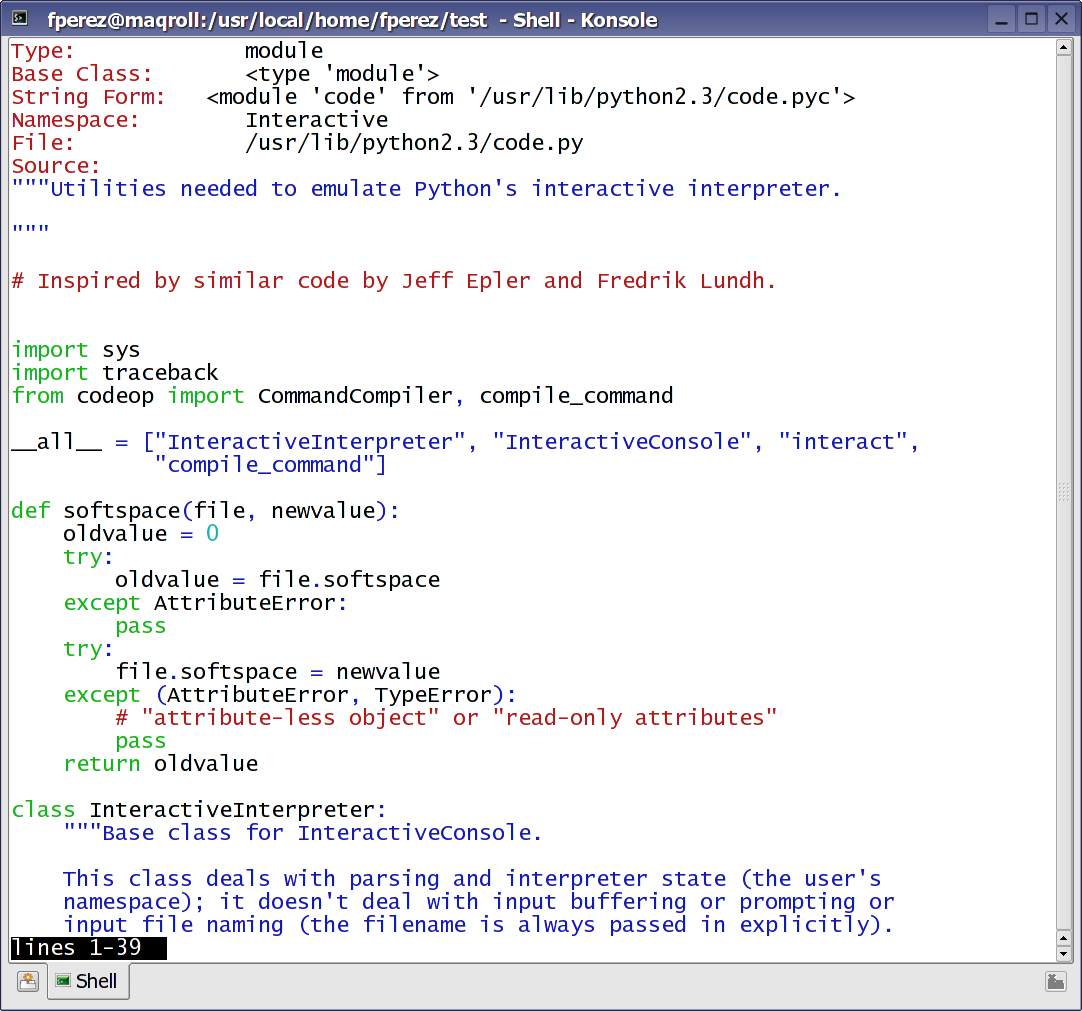
\includegraphics[width=0.48\linewidth]{fig/ipscr_code}~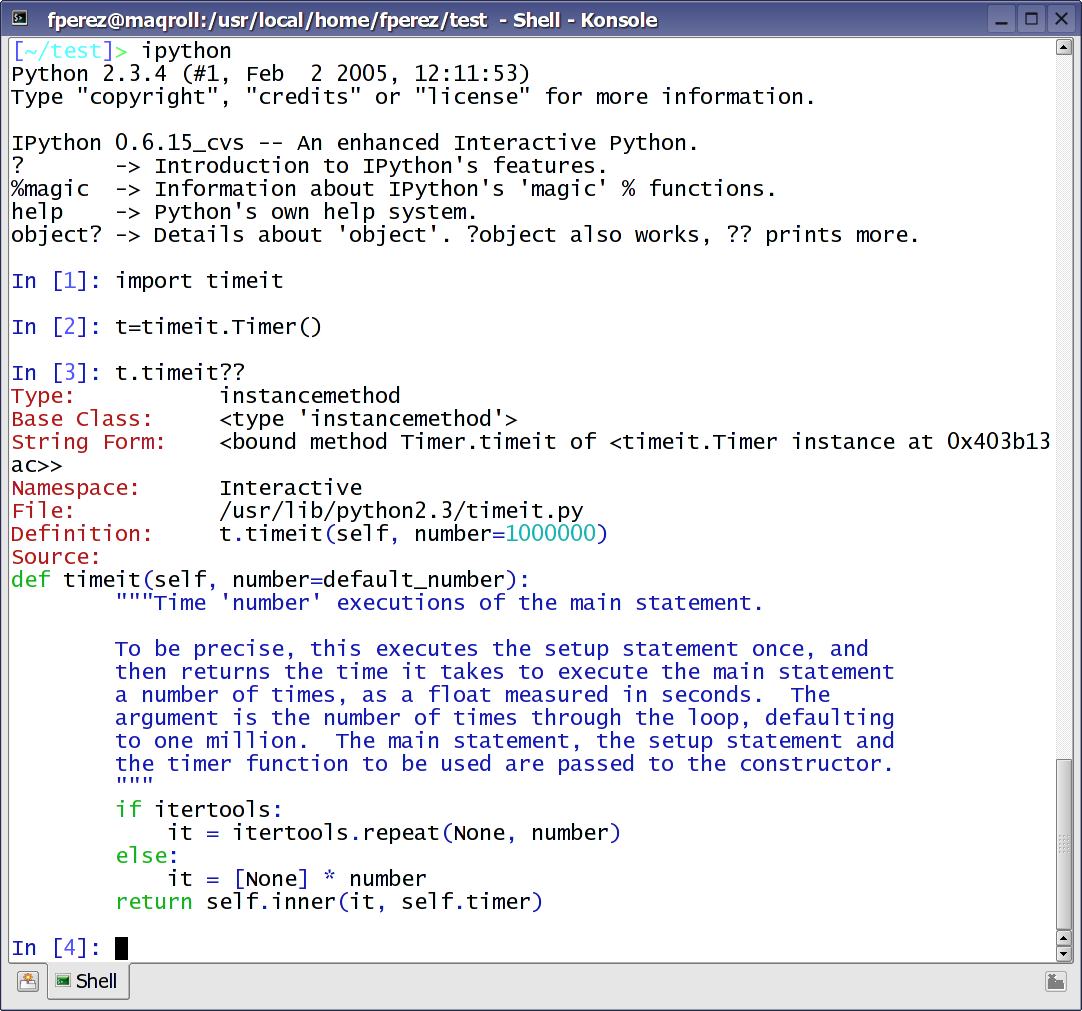
\includegraphics[width=0.48\linewidth]{fig/ipscr_meth_src}
\par\end{centering}

\caption{\label{fig:ipscr_code}IPython can show syntax-highlighted source
code for objects whose source is available.}

\end{figure}



\subsection{Input and Ouptut cached prompts}

In IPython, all output results are automatically stored in a global
dictionary named \texttt{Out} and variables named \texttt{\_1}, \texttt{\_2},
etc. alias them. For example, the result of input line 4 is available
either as \texttt{Out{[}4]} or as \texttt{\_4}. Additionally, three
variables named \texttt{\_}, \texttt{\_\_} and \texttt{\_\_\_} are
always kept updated with the for the last three results. This allows
you to recall any previous result and further use it for new calculations.
For example:

\begin{lyxcode}
In~{[}1]:~2+4

Out{[}1]:~6



In~{[}2]:~\_+9

Out{[}2]:~15



In~{[}3]:~\_+\_\_

Out{[}3]:~21



In~{[}4]:~print~\_1

6



In~{[}5]:~print~Out{[}1]

6



In~{[}6]:~\_2{*}{*}3

Out{[}6]:~3375
\end{lyxcode}
You can put a \texttt{`;}' at the end of a line to supress the printing
of output. This is useful when doing calculations which generate long
output you are not interested in seeing. The \texttt{\_{*}} variables
and the \texttt{Out{[}]} list do get updated with the contents of
the output, even if it is not printed. You can thus still access the
generated results this way for further processing.

A similar system exists for caching input. All input is stored in
a global list called \texttt{In} , so you can re-execute lines 22
through 28 plus line 34 by typing \texttt{'exec In{[}22:29]+In{[}34]'}
(using Python slicing notation). 

At any time, your input history remains available. The \texttt{\%hist}
command can show you all previous input, without line numbers if desired
(option \texttt{-n}) so you can directly copy and paste code either
back in IPython or in a text editor. You can also save all your history
by turning on logging via \texttt{\%logstart}; these logs can later
be either reloaded as IPython sessions or used as code for your programs.

If you need to execute the same set of lines often, you can assign
them to a macro with the \texttt{\%macro} magic function. Macros are
simply short names for groups of input lines, which can be re-executed
by only typing that name. Typing \texttt{macro?} at the prompt will
show you the function's full documentation. For example, if your history
contains:

\begin{lyxcode}
44:~x=1

45:~y=3

46:~z=x+y

47:~print~x

48:~a=5

49:~print~'x',x,'y',y
\end{lyxcode}
You can create a macro with lines 44 through 47 (included) and line
49 called \texttt{my\_macro} with:

\begin{lyxcode}
In~{[}51]:~\%macro~my\_macro~44:48~49
\end{lyxcode}
Now, simply typing \texttt{my\_macro} will re-execute all this code
in one pass. The number range follows standard Python list slicing
notation, where \texttt{n:m} means the numbers $(n,n+1,\ldots,m-1).$

You should note that macros execute in the current context, so if
any variable changes, the macro will pick up the new value every time
it is executed:

\begin{lyxcode}
In~{[}1]:~x=1

In~{[}2]:~y=x{*}5

In~{[}3]:~z=x+3

In~{[}4]:~print~'y~is:',y,'and~z~is:',z

y~is:~5~and~z~is:~4

\textcolor{blue}{\#~make~a~macro~with~lines~2,3,4~(note~Python~list~slice~syntax):}

In~{[}5]:~macro~yz~2:5

Macro~`yz`~created.~To~execute,~type~its~name~(without~quotes).

Macro~contents:

y=x{*}5

z=x+3

print~'y~is:',y,'and~z~is:',z

\textcolor{blue}{\#~now,~run~the~macro~directly:}

In~{[}6]:~yz

Out{[}6]:~Executing~Macro...

y~is:~5~and~z~is:~4

\textcolor{blue}{\#~we~change~the~value~of~x}

In~{[}7]:~x=9

\textcolor{blue}{\#~and~now~if~we~rerun~the~macro,~we~get~the~new~values:}

In~{[}8]:~yz

Out{[}8]:~Executing~Macro...

y~is:~45~and~z~is:~12
\end{lyxcode}

\subsection{Running code}

The \texttt{\%run} magic command allows you to run any python script
and load all of its data directly into the interactive namespace.
\texttt{\%run} is a sophisticated wrapper around the Python \texttt{execfile()}
builtin function; since the file is re-read from disk each time, changes
you make to it are reflected immediately (in contrast to the behavior
of \texttt{import}). I rarely use \texttt{import} for code I am testing,
relying on \texttt{\%run} instead. 

By default, 

\begin{lyxcode}
\%run~myfile~arg1~arg2~...
\end{lyxcode}
executes \texttt{myfile} in a namespace initially consisting only
of \texttt{\_\_name\_\_=='\_\_main\_\_'} and \texttt{sys.argv} being
filled with arg1, arg2, etc. This means that using \texttt{\%run}
is functionally very simlar to executing a script at the system command
line, but you get all the functionality of IPython (better tracebacks,
debugger and profiler access, etc.). The \texttt{-n} option prevents
\texttt{\_\_name\_\_} from being set equal to \texttt{'\_\_main\_\_'},
in case you want to test the part of a script which only runs when
\texttt{import}ed. 

Additionally, the fact that IPython then updates your interactive
namespace with the variables defined in the script is very useful,
because you can run your code to do a lot of processing, and then
continue using and exploring interactively the objects created by
the program. 

For example, if the file \texttt{ip\_simple.py} contains:

\lstinputlisting{examples/ip_simple.py}you can run it in IPython
as follows:

\begin{lyxcode}
\textcolor{blue}{\#~First,~let's~check~that~x~is~undefined}

In~{[}1]:~x

-{}-{}-{}-{}-{}-{}-{}-{}-{}-{}-{}-{}-{}-{}-{}-{}-{}-{}-{}-{}-{}-{}-{}-{}-{}-{}-{}-{}-{}-{}-{}-{}-{}-{}-{}-{}-{}-{}-{}-{}-{}-{}-{}-{}-{}-{}-{}-{}-{}-{}-{}-{}-{}-{}-{}-{}-{}-{}-{}-{}-{}-{}-{}-{}-{}-{}-{}-{}-{}-{}-{}-{}-{}-{}-

exceptions.NameError~~~~~~~~~~~~~~~~~~~~~~~~~~~~~~~~~Traceback~(most~recent~call~last)

/usr/local/home/fperez/teach/course/problems/<console>

NameError:~name~'x'~is~not~defined



\textcolor{blue}{\#~Now~we~run~the~script~(the~.py~extension~is~optional):}

In~{[}2]:~run~ip\_simple

sys.argv~is:~{[}'ip\_simple.py']

\_\_name\_\_~is:~\_\_main\_\_



\textcolor{blue}{\#~If~we~print~x,~now~it~has~the~value~from~the~script}

In~{[}3]:~x

Out{[}3]:~1



\textcolor{blue}{\#~Again,~but~now~running~with~some~arguments:}

In~{[}4]:~run~ip\_simple~-x~arg1~\char`\"{}hello~world\char`\"{}

sys.argv~is:~{[}'ip\_simple.py',~'-x',~'arg1',~'hello~world']

\_\_name\_\_~is:~\_\_main\_\_
\end{lyxcode}
With the \texttt{-i} option, the namespace where your script runs
is actually your interactive one. This can be used for two sligthly
different purposes. The simpler case, is just to quickly type up a
set of commands in an editor which you want to execute on your current
environment (although the \texttt{\%edit} command can also be used
for this). Consider running the file \texttt{ip\_simple2.py}:

\lstinputlisting{examples/ip_simple2.py}in IPython:

\begin{lyxcode}
\textcolor{blue}{\#~A~regular~\%run~will~produce~an~error:}

In~{[}1]:~run~ip\_simple2

-{}-{}-{}-{}-{}-{}-{}-{}-{}-{}-{}-{}-{}-{}-{}-{}-{}-{}-{}-{}-{}-{}-{}-{}-{}-{}-{}-{}-{}-{}-{}-{}-{}-{}-{}-{}-{}-{}-{}-{}-{}-{}-{}-{}-{}-{}-{}-{}-{}-{}-{}-{}-{}-{}-{}-{}-

exceptions.NameError~~~~~~~~~~~~~~Traceback~(most~recent~call~last)

/usr/local/home/fperez/teach/course/problems/ip\_simple2.py

~~~~~~2

~~~~~~3~It~should~be~run~via~IPython's~\%run~with~the~-i~option.\char`\"{}\char`\"{}\char`\"{}

~~~~~~4

-{}-{}-{}->~5~print~'x~is:',x

~~~~~~6

NameError:~name~'x'~is~not~defined

WARNING:~Failure~executing~file:~<ip\_simple2.py>

x~is:

\textcolor{blue}{\#~However,~if~you~do~have~a~variable~x~defined:}

In~{[}2]:~x='hello'

\textcolor{blue}{\#~you~can~use~the~-i~option~and~the~code~will~see~x:}

In~{[}3]:~run~-i~ip\_simple2

x~is:~hello
\end{lyxcode}
A different use of \texttt{\%run -i}, is to repeatedly run scripts
which may have a potentially expensive initialization phase. If this
initialization does not need to be repeated on each run (for example,
you are debugging some other submodule and can reuse the same expensive
object several times), you can avoid it by protecting the expensive
object with a \texttt{try/except} block. This simple script illustrates
the technique:

\lstinputlisting{examples/ip_expensive_init.py}In IPython, here is
how you can use it:

\begin{lyxcode}
\textcolor{blue}{\#~The~first~time~it~runs,~it~will~have~to~initialize}

In~{[}1]:~run~-i~ip\_expensive\_init.py

bigobject~not~found,~performing~expensive~initialization...

total~is:~499500

\textcolor{blue}{\#~but~successive~runs~don't~require~initialization}

In~{[}2]:~run~-i~ip\_expensive\_init.py

We~found~bigobject!~No~need~to~initialize~it.

total~is:~499500

\textcolor{blue}{\#~you~can~still~run~without~-i,~to~achieve~a~full~reload~}

\textcolor{blue}{\#~if~you~need~it~for~any~reason}

In~{[}3]:~run~ip\_expensive\_init.py

bigobject~not~found,~performing~expensive~initialization...

total~is:~499500
\end{lyxcode}
In the third run, by not using \texttt{-i}, your script runs in an
empty namespace and this forces a full initialization (the \texttt{NameError}
exception is triggered).

\texttt{\%run} also has special flags for timing the execution of
your scripts (\texttt{-t}) and for executing them under the control
of either Python's \texttt{pdb} debugger (\texttt{-d}) or profiler
(\texttt{-p}). You can get all of its docstring with the usual \texttt{run?}
mechanism.

Thanks to all of its various control options, \texttt{\%run} can be
used as the main tool for efficient interactive development of code
which you write in your editor of choice. My personal operation mode,
which has served me well for several years of scientific work in Python,
is to have a good editor (XEmacs in my case) open with all my Python
code, and IPython open in a terminal where I run, debug, explore,
plot, etc.


\section[OS access]{Access to the underlying Operating System}


\subsection{Basic usage}

IPython allows you to always access the underlying OS very easily.
Any lines starting with \texttt{!} are passed directly to the system
shell:

\begin{lyxcode}
In~{[}6]:~!ls~ip{*}.py

ip\_expensive\_init.py~~ip\_simple2.py~~ip\_simple.py
\end{lyxcode}
and using \texttt{!!} captures shell output into python variables
for further use:

\begin{lyxcode}
In~{[}7]:~!!ls~ip{*}.py

Out{[}7]:~{[}'ip\_expensive\_init.py',~'ip\_simple2.py',~'ip\_simple.py']
\end{lyxcode}
There is a difference between the two cases: in the first, the \texttt{ls}
command simply prints its results to the terminal as text, but no
value is returned. In the second, IPython actually captures the output
of the command, splits it as a list (one line per entry), and returns
its value. This allows you to then operate on the results with Python
routines.

Additionally, IPython plays a few interesting syntactic tricks for
your convenience. Whenever you make a system call, IPython will expand
any call of the type \texttt{\$var} into the actual value of the python
variable \texttt{var}, so that you can call shell commands on Python
values. Continuing the session above, and remembering that \texttt{\_}
holds the previously returned value, we can call the `\texttt{wc -l}'
Unix command (which does a line count on a file) on the files we just
obtained:

\begin{lyxcode}
In~{[}8]:~for~f~in~\_:

~~~...:~~~~~~if~'simple'~in~f:

~~~...:~~~~~~~~~~!wc~-l~\$f

~~~...:

3~ip\_simple2.py

4~ip\_simple.py
\end{lyxcode}
While this is completely unorthodox (actually, invalid) Python, it
is the kind of functionality which can make for extremely efficient
uses when working at an interactive command line. Obviously all of
this can be done (and it \emph{is} done that way by IPython internally)
with regular Python code, but that approach requires a fair amount
more typing, the use of \texttt{\%}-based string interpolation, and
making system calls via the \texttt{os.system()} function.

If you actually need to pass a \texttt{\$} character to a shell command,
you simply use \texttt{\$\$} in the IPython command line:

\begin{lyxcode}
In~{[}11]:~!echo~\$\$SHELL

/bin/tcsh
\end{lyxcode}
If you want to capture the output of a system command directly to
a named Python variable, you can use the \texttt{\%sc} magic function:

\begin{lyxcode}
\textcolor{blue}{\#~by~default,~\%sc~captures~to~a~plain~string:}

In~{[}16]:~\%sc~astr=ls~ip{*}.py

In~{[}17]:~astr

Out{[}17]:~'ip\_expensive\_init.py\textbackslash{}nip\_simple2.py\textbackslash{}nip\_simple.py'

\textcolor{blue}{\#~but~with~the~-l~option,~it~splits~to~a~list~(like~!!~does)}

In~{[}18]:~\%sc~-l~alist=ls~ip{*}.py

In~{[}19]:~alist

Out{[}19]:~{[}'ip\_expensive\_init.py',~'ip\_simple2.py',~'ip\_simple.py']
\end{lyxcode}

\subsection{System aliases}

In IPython, you can also define your own system aliases. Even though
IPython gives you access to your system shell via the \texttt{!} prefix,
it is convenient to have aliases to the system commands you use most
often. This allows you to work seamlessly from inside IPython with
the same commands you are used to in your system shell:

\texttt{`\%alias alias\_name cmd'} defines \texttt{`alias\_name'}
as an alias for \texttt{`cmd'}

Then, typing \texttt{`alias\_name params'} will execute the system
command \texttt{`cmd params'} (from your underlying operating system).
Aliases have lower precedence than magic functions and Python normal
variables, so if \texttt{`foo'} is both a Python variable and an alias,
the alias can not be executed until \texttt{`del foo'} removes the
Python variable. If you need to access an alias directly, you can
use the builtin function \texttt{ipalias} as \texttt{ipalias('foo')}.

You can use the \texttt{\%l} specifier in an alias definition to represent
the whole line when the alias is called. For example:

\begin{lyxcode}
In~{[}2]:~alias~all~echo~\char`\"{}Input~in~brackets:~<\%l>\char`\"{}

In~{[}3]:~all~hello~world

Input~in~brackets:~<hello~world>
\end{lyxcode}
You can also define aliases with positional parameters using \texttt{\%s}
specifiers (one per parameter):

\begin{lyxcode}
In~{[}1]:~alias~parts~echo~first~\%s~second~\%s

In~{[}2]:~\%parts~A~B

first~A~second~B

In~{[}3]:~\%parts~A

Incorrect~number~of~arguments:~2~expected.

parts~is~an~alias~to:~'echo~first~\%s~second~\%s'
\end{lyxcode}
Aliases expand Python variables just like system calls using \texttt{!}
or \texttt{!!} do: all expressions prefixed with '\texttt{\$}' get
expanded. For details of the semantic rules, see PEP-215: \url{http://www.python.org/peps/pep-0215.html}.
This is the library used by IPython for variable expansion.

Simply typing \texttt{alias} will print a list of the current aliases,
and \texttt{unalias} can be used to remove an alias. For further details,
use \texttt{alias?}.


\subsection{Directory management}

IPython comes with some pre-defined aliases and a complete system
for changing directories, both via a stack (see \texttt{\%pushd},
\texttt{\%popd} and \texttt{\%ds}) and via direct \texttt{\%cd}. The
latter keeps a history of visited directories and allows you to go
to any previously visited one. You can see this history with the \texttt{\%dhist}
magic:

\begin{lyxcode}
In~{[}1]:~cd~\textasciitilde{}/code/python

/home/fperez/code/python

In~{[}2]:~cd~\textasciitilde{}/teach/

/home/fperez/teach

In~{[}3]:~cd~\textasciitilde{}/research

/home/fperez/research

In~{[}4]:~dhist

Directory~history~(kept~in~\_dh)

0:~/home/fperez/teach/course/examples

1:~/home/fperez/code/python

2:~/home/fperez/teach

3:~/home/fperez/research

In~{[}5]:~cd~-1

/home/fperez/code/python
\end{lyxcode}
The \texttt{\%bookmark} magic allows you to create named bookmarks
in your filesystem, which \texttt{cd} can be directed to go to (with
the \texttt{-b} flag), and to which it will try to default automatically
if no such named directory exists. The system is very easy to use
and quite natural in practice:

\begin{lyxcode}
In~{[}8]:~bookmark~course

In~{[}9]:~cd

/home/fperez

In~{[}10]:~ls~course

ls:~course:~No~such~file~or~directory

In~{[}11]:~cd~course

(bookmark:course)~->~/home/fperez/teach/course

/home/fperez/teach/course
\end{lyxcode}

\subsection{IPython as a system shell}

While IPython is \emph{not} a system shell, it ships with a special
profile called \texttt{pysh}, which you can activate at the command
line as \texttt{`ipython -p pysh'}. This modifies IPython's behavior
and adds some additional facilities and a prompt customized for filesystem
navigation.

Note that this does \emph{not} make IPython a full-fledged system
shell. In particular, it has no job control, so if you type Ctrl-Z
(under Unix), you'll suspend pysh itself, not the process you just
started. 

What the shell profile allows you to do is to use the convenient and
powerful syntax of Python to do quick scripting at the command line.
Below we describe some of its features.


\subsubsection{Aliases}

All of your \texttt{\$PATH} has been loaded as IPython aliases, so
you should be able to type any normal system command and have it executed.
See \texttt{\%alias?} and \texttt{\%unalias?} for details on the alias
facilities. See also \texttt{\%rehash?} and \texttt{\%rehashx?} for
details on the mechanism used to load \texttt{\$PATH}.


\subsubsection{Special syntax}

Any lines which begin with \texttt{`\textasciitilde{}'}, \texttt{`/'}
and \texttt{`.'} will be executed as shell commands instead of as
Python code. The special escapes below are also recognized. \texttt{!cmd}
is valid in single or multi-line input, all others are only valid
in single-line input:

\begin{description}
\item [{\texttt{!cmd}}] pass `cmd' directly to the shell 
\item [{\texttt{!!cmd}}] execute `cmd' and return output as a list (split
on `\textbackslash{}n') 
\item [{\texttt{\$var=cmd}}] capture output of cmd into var, as a string
(shorthand for \texttt{\%sc var=cmd})
\item [{\texttt{\$\$var=cmd}}] capture output of cmd into var, as a list
(split on `\textbackslash{}n', shorthand for \texttt{\%sc -l var=cmd})
\end{description}

\subsubsection{Useful functions and modules}

The os, sys and shutil modules from the Python standard library are
automatically loaded. Some additional functions, useful for shell
usage, are listed below. You can request more help about them with
`\texttt{?}'.

\begin{description}
\item [{\texttt{shell}}] - execute a command in the underlying system shell 
\item [{\texttt{system}}] - like \texttt{shell()}, but return the exit
status of the command
\item [{\texttt{sout}}] - capture the output of a command as a string
\item [{\texttt{lout}}] - capture the output of a command as a list (split
on `\textbackslash{}n')
\item [{\texttt{getoutputerror}}] - capture (output,error) of a shell commandss
\end{description}
\texttt{sout}/\texttt{lout} are the functional equivalents of \texttt{\$}/\texttt{\$\$}.
They are provided to allow you to capture system output in the middle
of true python code, function definitions, etc (where \texttt{\$}
and \texttt{\$\$} are invalid)


\section{Access to an editor}

You can use \texttt{\%edit} to have almost multiline editing. While
IPython doesn't support true multiline editing, this command allows
you to call an editor on the spot, and IPython will execute the code
you type in there as if it were typed interactively. 

\texttt{\%edit} runs your IPython configured editor. By default this
is read from your environment variable \texttt{\$EDITOR}. If this
isn't found, it will default to \texttt{vi} under Linux/Unix and to
\texttt{notepad} under Windows. 

You can also set the value of this editor via the command-line option
\texttt{`-editor'} or in your \texttt{ipythonrc} file. This is useful
if you wish to use specifically for IPython an editor different from
your typical default (and for Windows users who typically don't set
environment variables).

This command allows you to conveniently edit multi-line code right
in your IPython session.

If called without arguments, \texttt{\%edit} opens up an empty editor
with a temporary file and will execute the contents of this file when
you close it (don't forget to save it!). 


\section{Customizing IPython}


\subsection{Basics}

IPython has a very flexible configuration system. It uses a configuration
file which allows permanent setting of all command-line options, module
loading, code and file execution. The system allows recursive file
inclusion, so you can have a base file with defaults and layers which
load other customizations for particular projects.

IPython reads a configuration file which can be specified at the command
line (\texttt{-rcfile}) or which by default is assumed to be called
\texttt{ipythonrc}. Such a file is looked for in the current directory
where IPython is started and then in your \texttt{IPYTHONDIR}, which
allows you to have local configuration files for specific projects.
The default value for this directory is \texttt{\$HOME/.ipython} (\texttt{\_ipython}
under Windows). Under Unix operating systems \texttt{\$HOME} always
exists; for Windows, IPython will try to find such an environment
variable; if it doesn't exist, it uses \texttt{HOMEDRIVE\textbackslash{}HOMEPATH}
(these are always defined by Windows). This typically gives something
like \texttt{C:\textbackslash{}Documents and Settings\textbackslash{}YourUserName},
but your local details may vary. Finally, you can make this directory
live anywhere you want by creating an environment variable called
\texttt{\$IPYTHONDIR}.

In this directory you will find all the files that configure IPython's
defaults, and you can put there your profiles and extensions. This
directory is automatically added by IPython to \texttt{sys.path},
so anything you place there can be found by \texttt{import} statements.

The syntax of an rcfile is one of key-value pairs separated by whitespace,
one per line. Lines beginning with a \texttt{\#} are ignored as comments,
but comments can \textbf{not} be put on lines with data (the parser
is fairly primitive). You can study the default rcfile created by
IPython at startup for customization details, it is extremely commented.


\subsection{Profiles}

IPython can load any configuration file you want if you give its name
at startup with the \texttt{-rcfile} flag. However, for convenience
it provides a shorthand based on a naming convention for loading such
profiles. This system allows you to easily maintain customized versions
of IPython for specific purposes.

With the \texttt{-profile <name>} flag (you can abbreviate it to \texttt{-p}),
IPython will assume that your config file is called \texttt{ipythonrc-<name>}
(it looks in current dir first, then in \texttt{IPYTHONDIR}). This
is a quick way to keep and load multiple config files for different
tasks, especially if you use the include option of config files. You
can keep a basic \texttt{IPYTHONDIR/ipythonrc} file and then have
other profiles which include this one and load extra things for particular
tasks. For example:

\begin{enumerate}
\item \texttt{\$HOME/.ipython/ipythonrc}: load basic things you always want. 
\item \texttt{\$HOME/.ipython/ipythonrc-math}: load (1) and basic math-related
modules. 
\item \texttt{\$HOME/.ipython/ipythonrc-numeric}: load (1) and Numeric and
plotting modules.
\end{enumerate}
Since it is possible to create an endless loop by having circular
file inclusions, IPython will stop if it reaches 15 recursive inclusions.


\section[Debugging and profiling]{Debugging and profiling with IPython }

The Python standard library includes powerful facilities for debugging
and profiling code, but it is common to find even experienced Python
programmers who still do not take advantage of them. In part, this
is due to the fact that loading and configuring them requires reading
an extra documentation section, and keeping a bit of additional information
about their use in your head. IPython tries to automate their use
to the point where, with a single command, you can use either of these
subsystems in a transparent manner. Hopefully they will become part
of your daily workflow.

At its most basic, for debugging your programs, you can rely on using
\texttt{\%run} to execute them, see the results, play with all variables
loaded into the interactive namespace, etc. A typical working session
involves keeping your favorite editor open with the file you are working
on, and repeatedly calling \texttt{\%run} on it as you make changes
and save them.

%
\begin{figure}
\begin{centering}
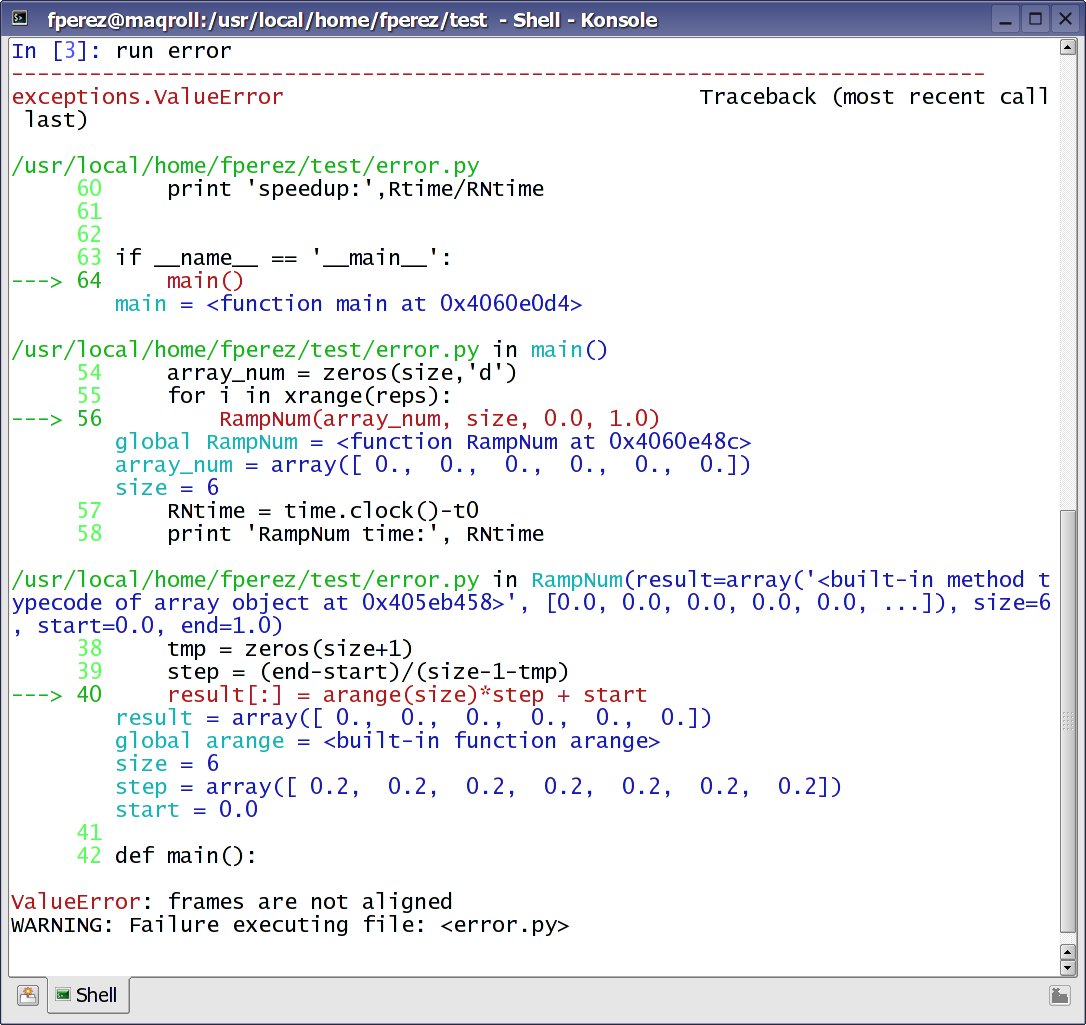
\includegraphics[width=0.7\linewidth]{fig/ipscr_traceback}
\par\end{centering}

\caption{\label{fig:ipscr_traceback}IPython can provide extremely detailed
tracebacks.}

\end{figure}


If your program raises an exception, IPython will provide you with
a more detailed traceback than the default Python ones. You can even
increase the level of detail further by using \texttt{\%xmode Verbose},
which forces the printing of variable values at all stack frames.
This option should be used with care though (and that's why it is
not the default), as printing a ten-million-entry array can lock up
your computer for a very long time. An example of this kind of very
informative traceback is shown in Fig.~\ref{fig:ipscr_traceback}.


\subsection{Automatic invocation of \texttt{pdb} on exceptions}

IPython, if started with the \texttt{-pdb} option (or if the option
is set in your rc file) can call the Python \texttt{pdb} debugger
every time your code triggers an uncaught exception. This feature
can also be toggled at any time with the \texttt{\%pdb} magic command.
This can be extremely useful in order to find the origin of subtle
bugs, because \texttt{pdb} opens up at the point in your code which
triggered the exception, and while your program is at this point `dead',
all the data is still available and you can walk up and down the stack
frame and understand the origin of the problem.

Furthermore, you can use these debugging facilities both with the
embedded IPython mode and without IPython at all. For an embedded
shell (see sec. \ref{sec:ipython_embed}), simply call the constructor
with \texttt{`-pdb'} in the argument string and automatically \texttt{pdb}
will be called if an uncaught exception is triggered by your code. 

For stand-alone use of the feature in your programs which do not use
IPython at all, put the following lines toward the top of your `main'
routine:

\begin{lyxcode}
import~sys,IPython.ultraTB

sys.excepthook~=~IPython.ultraTB.FormattedTB(mode=`Verbose',~~\\
color\_scheme=`Linux',~call\_pdb=1)
\end{lyxcode}
The \texttt{mode} keyword can be either \texttt{`Verbose'} or \texttt{`Plain'},
giving either very detailed or normal tracebacks respectively. The
\texttt{color\_scheme} keyword can be one of \texttt{`NoColor'}, \texttt{`Linux'}
(default) or \texttt{`LightBG'}. These are the same options which
can be set in IPython with \texttt{-colors} and \texttt{-xmode}.

This will give any of your programs detailed, colored tracebacks with
automatic invocation of \texttt{pdb}.


\subsection{Running entire programs via \texttt{pdb}}

\texttt{pdb}, the Python debugger, is a powerful interactive debugger
which allows you to step through code, set breakpoints, watch variables,
etc. IPython makes it very easy to start any script under the control
of \texttt{pdb}, regardless of whether you have wrapped it into a
\texttt{`main()'} function or not. For this, simply type \texttt{`\%run
-d myscript'} at an IPython prompt. See the \texttt{\%run} command's
documentation (\texttt{run?}) for more details, including how to control
where \texttt{pdb} will stop execution first.

For more information on the use of the \texttt{pdb} debugger, read
the included \texttt{pdb.doc} file (part of the standard Python distribution).
On a stock Linux system it is located at \texttt{/usr/lib/python2.3/pdb.doc},
but the easiest way to read it is by using the \texttt{help()} function
of the \texttt{pdb} module as follows (in an IPython prompt):

\begin{lyxcode}
In~{[}1]:~import~pdb

In~{[}2]:~pdb.help()
\end{lyxcode}
This will load the \texttt{pdb.doc} document in a file viewer for
you automatically.


\subsection{Profiling}

When dealing with performance issues, the \texttt{\%run} command with
a \texttt{-p} option allows you to run complete programs under the
control of the Python profiler. The \texttt{\%prun} command does a
similar job for single Python expressions (like function calls, similar
to \texttt{profile.run()}). While this is possible with the standard
\texttt{profile} module, IPython wraps this functionality with magic
commands convenient for rapid interactive work.


\section[Embedding]{\label{sec:ipython_embed}Embedding IPython into your programs }

A few lines of code are enough to load a complete IPython inside your
own programs, giving you the ability to work with your data interactively
after automatic processing has been completed. 

You can call IPython as a python shell inside your own python programs.
This can be used both for debugging code or for providing interactive
abilities to your programs with knowledge about the local namespaces
(very useful in debugging and data analysis situations).

It is possible to start an IPython instance \emph{inside} your own
Python programs. This allows you to evaluate dynamically the state
of your code, operate with your variables, analyze them, etc. Note
however that any changes you make to values while in the shell do
\emph{not} propagate back to the running code, so it is safe to modify
your values because you won't break your code in bizarre ways by doing
so.

This feature allows you to easily have a fully functional python environment
for doing object introspection anywhere in your code with a simple
function call. In some cases a simple print statement is enough, but
if you need to do more detailed analysis of a code fragment this feature
can be very valuable.

It can also be useful in scientific computing situations where it
is common to need to do some automatic, computationally intensive
part and then stop to look at data, plots, etc%
\footnote{This functionality was inspired by IDL's combination of the \texttt{stop}
keyword and the \texttt{.continue} executive command, which I have
found very useful in the past, and by a posting on comp.lang.python
by cmkl <cmkleffner@gmx.de> on Dec. 06/01 concerning similar uses
of pyrepl.%
}. Opening an IPython instance will give you full access to your data
and functions, and you can resume program execution once you are done
with the interactive part (perhaps to stop again later, as many times
as needed).

The following code snippet is the bare minimum you need to include
in your Python programs for this to work (detailed examples follow
later):

\begin{lyxcode}
from~IPython.Shell~import~IPShellEmbed

ipshell~=~IPShellEmbed()

ipshell()~\#~this~call~anywhere~in~your~program~will~start~IPython
\end{lyxcode}
You can run embedded instances even in code which is itself being
run at the IPython interactive prompt with '\texttt{\%run~<filename>}'.
Since it's easy to get lost as to where you are (in your top-level
IPython or in your embedded one), it's a good idea in such cases to
set the in/out prompts to something different for the embedded instances.
The code examples below illustrate this.

You can also have multiple IPython instances in your program and open
them separately, for example with different options for data presentation.
If you close and open the same instance multiple times, its prompt
counters simply continue from each execution to the next.

Please look at the docstrings in the \texttt{Shell.py} module for
more details on the use of this system.

The following sample file illustrating how to use the embedding functionality
is provided in the examples directory as \texttt{example-embed.py}.
It should be fairly self-explanatory:

\lstinputlisting{examples/ip_embed.py}

Once you understand how the system functions, you can use the following
code fragments in your programs which are ready for cut and paste:

\lstinputlisting{examples/ip_embed-short.py}


\section[Matplotlib]{\label{sec:ipython_pylab}Integration with Matplotlib}

The matplotlib library (\url{http://matplotlib.sourceforge.net})
provides high quality 2D plotting for Python. Matplotlib can produce
plots on screen using a variety of GUI toolkits, including Tk, GTK
and WXPython. It also provides a number of commands useful for scientific
computing, all with a syntax compatible with that of the popular Matlab
program.

IPython accepts the special option \texttt{-pylab}. This configures
it to support matplotlib, honoring the settings in the \texttt{.matplotlibrc}
file. IPython will detect the user's choice of matplotlib GUI backend,
and automatically select the proper threading model to prevent blocking.
It also sets matplotlib in interactive mode and modifies \texttt{\%run}
slightly, so that any matplotlib-based script can be executed using
\texttt{\%run} and the final \texttt{show()} command does not block
the interactive shell.

The \texttt{-pylab} option must be given first in order for IPython
to configure its threading mode. However, you can still issue other
options afterwards. This allows you to have a matplotlib-based environment
customized with additional modules using the standard IPython profile
mechanism: ``\texttt{ipython -pylab -p myprofile}'' will load the
profile defined in \texttt{ipythonrc-myprofile} after configuring
matplotlib.
